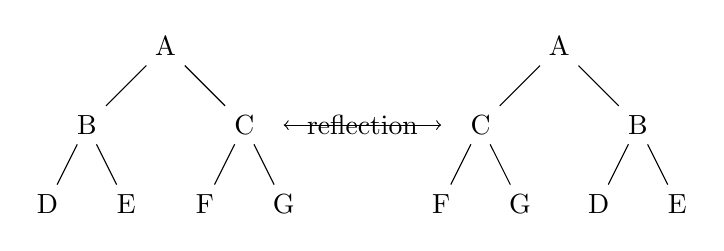
\begin{tikzpicture}
  \node (A) at (0,0) {A};
  \node (B) at (-1,-1) {B};
  \node (C) at ( 1,-1) {C};
  \node (D) at (-1.5,-2) {D};
  \node (E) at (-0.5,-2) {E};
  \node (F) at ( 0.5,-2) {F};
  \node (G) at ( 1.5,-2) {G};
  \draw
  (A) -- (B)
  (A) -- (C)
  (B) -- (D)
  (B) -- (E)
  (C) -- (F)
  (C) -- (G);
  \draw[<->] (1.5,-1) -- node {reflection} (3.5,-1);
  \begin{scope}[shift={(5,0)}]
  \node (A') at (0,0) {A};
  \node (B') at ( 1,-1) {B};
  \node (C') at (-1,-1) {C};
  \node (D') at ( 0.5,-2) {D};
  \node (E') at ( 1.5,-2) {E};
  \node (F') at (-1.5,-2) {F};
  \node (G') at (-0.5,-2) {G};
  \draw
  (A') -- (B')
  (A') -- (C')
  (B') -- (D')
  (B') -- (E')
  (C') -- (F')
  (C') -- (G');
  \end{scope}
\end{tikzpicture}

%%% Local Variables:
%%% mode: latex
%%% TeX-master: "../Master"
%%% End:
